% $Date$
% $Revision$
% $Author$

% !TEX root = SMV_Technical_Reference_Guide.tex

% -------------------  Introduction ------------------------

\section{Introduction}
This note discusses some of the physics and associated numerical
algorithms used by Smokeview~\cite{Smokeview_Users_Guide} to
visualize smoke and fire.  Smoke color and opacity are visualized
using quantitative physics based methods.  Flame color
is visualized using an arbitrary user specified color palette
where color is mapped to gas temperature.
Smoke opacity is visulized using Beer's law relating smoke density and opacity.

Realistic visualization of fire calculation methods are important
for applications where one wishes to observe qualitative effects
of fire and smoke rather than determine quantitative
characteristics of data such as temperature or velocity.  This
would be the case for a fire fighter using a computer based fire
fighting simulator. Realistic visualization methods, however,
complement but do not replace other more traditional visualization
methods such as 2D contouring or 3D iso-surfacing which are better
suited for quantitatively analyzing data.

Complete methods for visualizing smoke and fire data taking into
account interactions between light and smoke require the solution
of the radiation transport equation (RTE)~\cite{Siegel:2001} also
called the volume rendering equation in visualization
literature.~\cite{levoy:1988} This equation models how light is
affected after interacting with smoke, a participating medium. In
particular, Smokeview uses the RTE to account for extinction
(absorption plus out-scattering) by the smoke and emission from
the fire.

The form of the RTE used by Smokeview to model smoke and fire
appearance is identical to that used by FDS to model radiative
heat transfer. Smokeview uses an extinction coefficient
appropriate for visible light while FDS use one appropriate for
infrared wavelengths of light.  With the proper extinction
coefficient, however, Smokeview can also view smoke at other
wavelengths, simulating a thermal imager, for example. Smokeview
solves the RTE assuming a gray gas environment. This is the
default solution method for FDS. One other important difference is
that Smokeview requires a solution at only one point at a time
(any arbitrary point though), the observer's viewpoint, while FDS
requires a radiation field, a solution at all points within the
solution domain.
Approximations are
required in order to display smoke and fire at interactive frame
rates.  The primary approximation is to take advantage of the low
albedo character of smoke allowing one to either simplify or
eliminate scattering terms in the RTE.

A slice rendering method for the solving to the RTE,  splits the
integration path at grid planes within a 3D mesh.
A series of partially transparent slices are drawn through the data where each
slice is approximately perpendicular to the line of sight.
These partially transparent slice planes are then drawn
individually and combined by the video hardware to form one image.
The spacing of data within one plane and the spacing between planes are parameters
that can be specified by the user in order to speed up the visualization.

As the separation distance between slice planes becomes smaller, the
computed opacity values are subject to increased round off error
due to finite precision arithmetic.  In fact, if these planes are
sufficiently close, the computed opacities truncate to zero.   In
this situation other techniques for visualizing smoke such as volume rendering methods are required.

% -------------------  Radiation Transport Equation ------------------------

\section{Radiation Transport Equation}
The model used here to visualize smoke is the radiation transport
equation (RTE)~\cite{Siegel:2001}.  This equation uses radiance to
represent smoke appearance.  Radiance has units of Watts per
square meter per unit solid angle~\si{W/(sr.m^2)}.  The solid
angle accounts for the fact that a light source appears brighter
if it emits a given amount of light through a smaller
cross-sectional area.  Similarly the radiance of a light source does not
depend on distance from the
observer (unless a participating medium is present to absorb or
scatter  light) since any increase in distance that would reduce radiance is offset
by the light source's reduced cross sectional areal.
The radiation transport equation discussed in
this section models the change in radiance due to these factors.

\renewcommand{\dx}[1]{\,\mbox{d}#1}
\newcommand{\siga}{ \sigma_a(x) }
\newcommand{\sigt}{ \sigma_t(x) }
\newcommand{\sigs}{ \sigma_s(x) }
\newcommand{\sigts}{ \sigma_t(s) }
\newcommand{\Le}{ C_e(x) }
\newcommand{\Lexo}{ C_e(x,\omega) }
\newcommand{\Lxo}{ C(x,\omega) }
\newcommand{\dLdx}{ \frac{\dx{C}}{\dx{x}}(x)}
\newcommand{\intf}[2]{ \exp\left({\int_{#1}^{#2} \sigts \dx{s}}\right) }
\newcommand{\intff}[2]{ {\int_{#1}^{#2} \sigts \dx{s}} }
\newcommand{\intmf}[2]{ \exp\left({-\int_{#1}^{#2} \sigts \dx{s}}\right) }
\newcommand{\intmff}[2]{ {-\int_#1^#2 \sigts \dx{s}} }
\newcommand{\ddx}{ \frac{\mbox{d}}{\dx{x}} }

The radiation transport equation is used to calculate radiance due
to one or more light sources within a region possibly containing a
participating medium such as smoke~\cite{Siegel:2001}. The change
in radiance along a ray with direction $\omega$ at any one instant
and wavelength may be expressed using

\begin{eqnarray}
\label{eq:fullrte}
 \left(\omega\cdot\nabla\right)\Lxo =
-\underbrace{\siga\Lxo}_\mathrm{absorption}-\underbrace{\sigs\Lxo}_\mathrm{out-scattering}
+ \underbrace{\siga\Lexo}_\mathrm{emission} +
\underbrace{\sigs\int_{4\pi}p(x,\omega,\omega')C_i(x,\omega')\dx{\omega'}}_\mathrm{in-scattering}
\end{eqnarray}

\noindent where  $\Lxo$ represents the  radiance at $x$ along a
direction $\omega$. As illustrated in Fig. \ref{figRadiance}, the
right hand side of (\ref{eq:fullrte}) is split into four
components accounting for absorption, in and out scattering and
emission where $\siga$ is the absorption coefficient, $\sigs$ is
the scattering coefficient, $\Lexo$ is the radiance emitted at $x$
along a direction $\omega$ and $p(x,\omega,\omega')$ is the
fraction of light moving along direction $\omega'$ scattered along
direction $\omega$. Absorption and out-scattering cause radiance
to decrease while emission and in-scattering cause radiance to
increase. The radiance terms $C$, $C_e$ and $C_i$ have units of
\si{W/(m^2.sr)}. The coefficients $\sigma_a$ and $\sigma_s$ have
units of \si{1/m} and specify the time and location dependent
change per unit length to the radiance term to which they are
applied.

\begin{figure}[bph]
\begin{center}
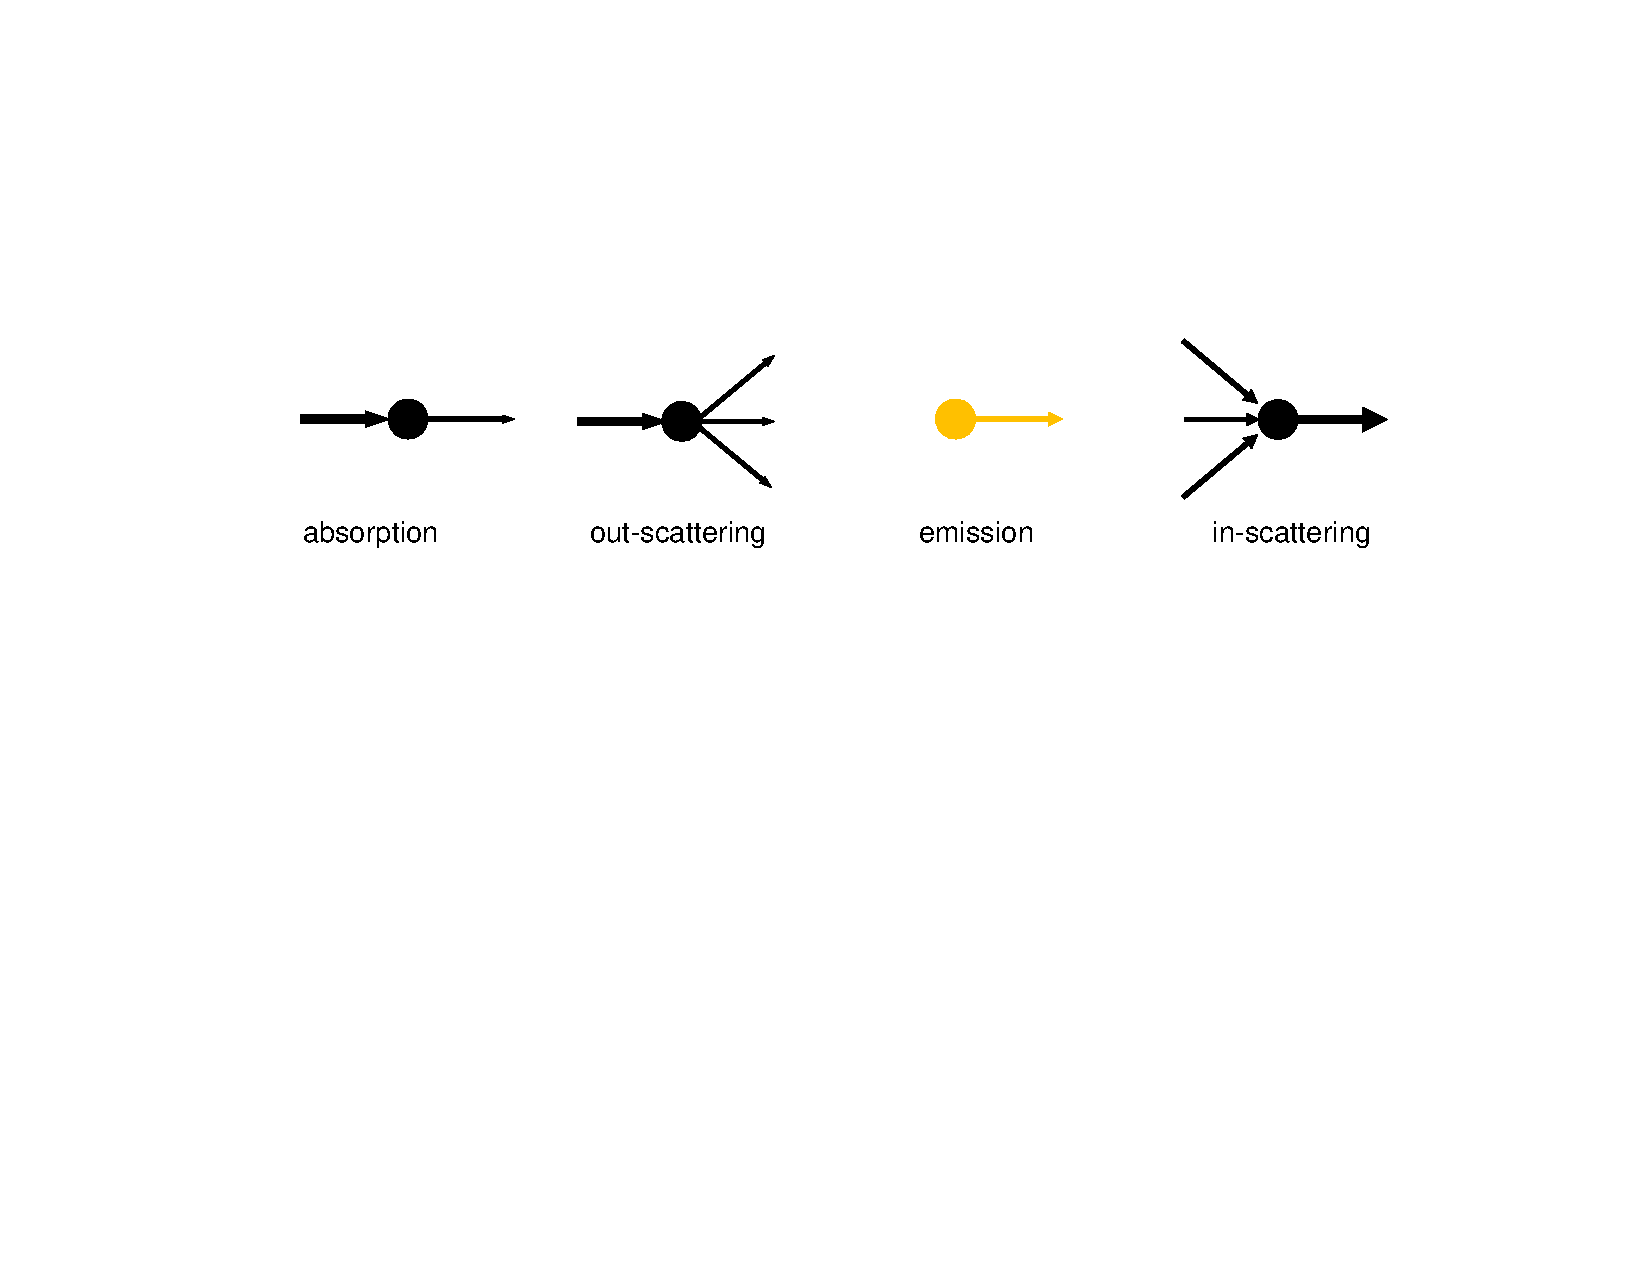
\includegraphics[width=6.0in]{\SMVfigdir/rte_setup}
\end{center}
\caption[Diagram illustrating components of the radiation
transport equation]{Diagram illustrating components of the
radiation transport equation.  Absorption and out-scattering terms
decrease radiance.  Emission and in-scattering terms increase
radiance.} \label{figRadiance}
\end{figure}

% ----  Approximating the Radiation Transport Equation ------------------------

\subsection{Approximating the Radiation Transport Equation}

The RTE may be simplified by ignoring the in-scattering term and combining out-scattering
and absorption coefficients.  The Beer-Lambert law results if the emission term is also
neglected.

Equation (\ref{eq:fullrte}) is then approximated by neglecting the
integral term and using $\sigt=\siga+\sigs$ to obtain

\begin{eqnarray}
\dLdx&=&-\sigt C(x) + \siga C_e(x)\\
 C(x_0)&=&C_0
\end{eqnarray}

\noindent This equation has solution

\begin{equation}
\label{eq:rtesoln}
 C(x_N)=\tau(x_0,x_N)C_0 + \int_{x_0}^{x_N}\tau(x,x_N)\siga\Le \dx{x}
\end{equation}

\noindent where $\tau(a,b)$ representing the optical depth between $a$ and $b$ is given by
\begin{equation}
\label{eq:optdepth}
\tau(a,b)=\intmf{a}{b}
\end{equation}

\noindent If the emission term is neglected and $\sigma_t(x)=\sigma_t$ is constant then this equation simplifies to
\begin{eqnarray}
 \frac{C(x_N)}{C_0}=\exp(-\sigma_tL)
\end{eqnarray}
which is the Beer-Lambert law.

% -------------------  Discretizing the Radiation Transport Equation ------------------------

\subsection{Discretizing the Radiation Transport Equation}
\newcommand{\htau}[1]{\tau_{#1}^{N-1}}
\newcommand{\halpha}[1]{\alpha_{#1}^{N-1}}
\newcommand{\sigai}[1]{\sigma_{a,#1}}
\newcommand{\Lei}[1]{C_{e,#1}}
\newcommand{\Lhatj}[1]{C_{#1}^N}
\newcommand{\Lhatjj}[1]{\hat{C}_{#1}^N}
\newcommand{\Chatjj}[1]{\hat{C}_{#1}^N}
\newcommand{\Leii}[1]{\hat{C}_{e,#1}}

The approximate RTE solution given in (\ref{eq:rtesoln}) is
discretized by converting integral into a sums Figure
\ref{fig:smokediscretesetup}\ illustrates the terms used to
perform these discretizations.  The path is split into $N$ parts
each with length $\Delta x=(x_N-x_0)/N$.  The coordinate system is
set up so that the initial radiance, $C_0$, is located at $x_0$,
most distant from the observer and the final radiance, $C_N$, is
located at $x_N$ closest to the observer.

\begin{figure}[bph]
\begin{center}
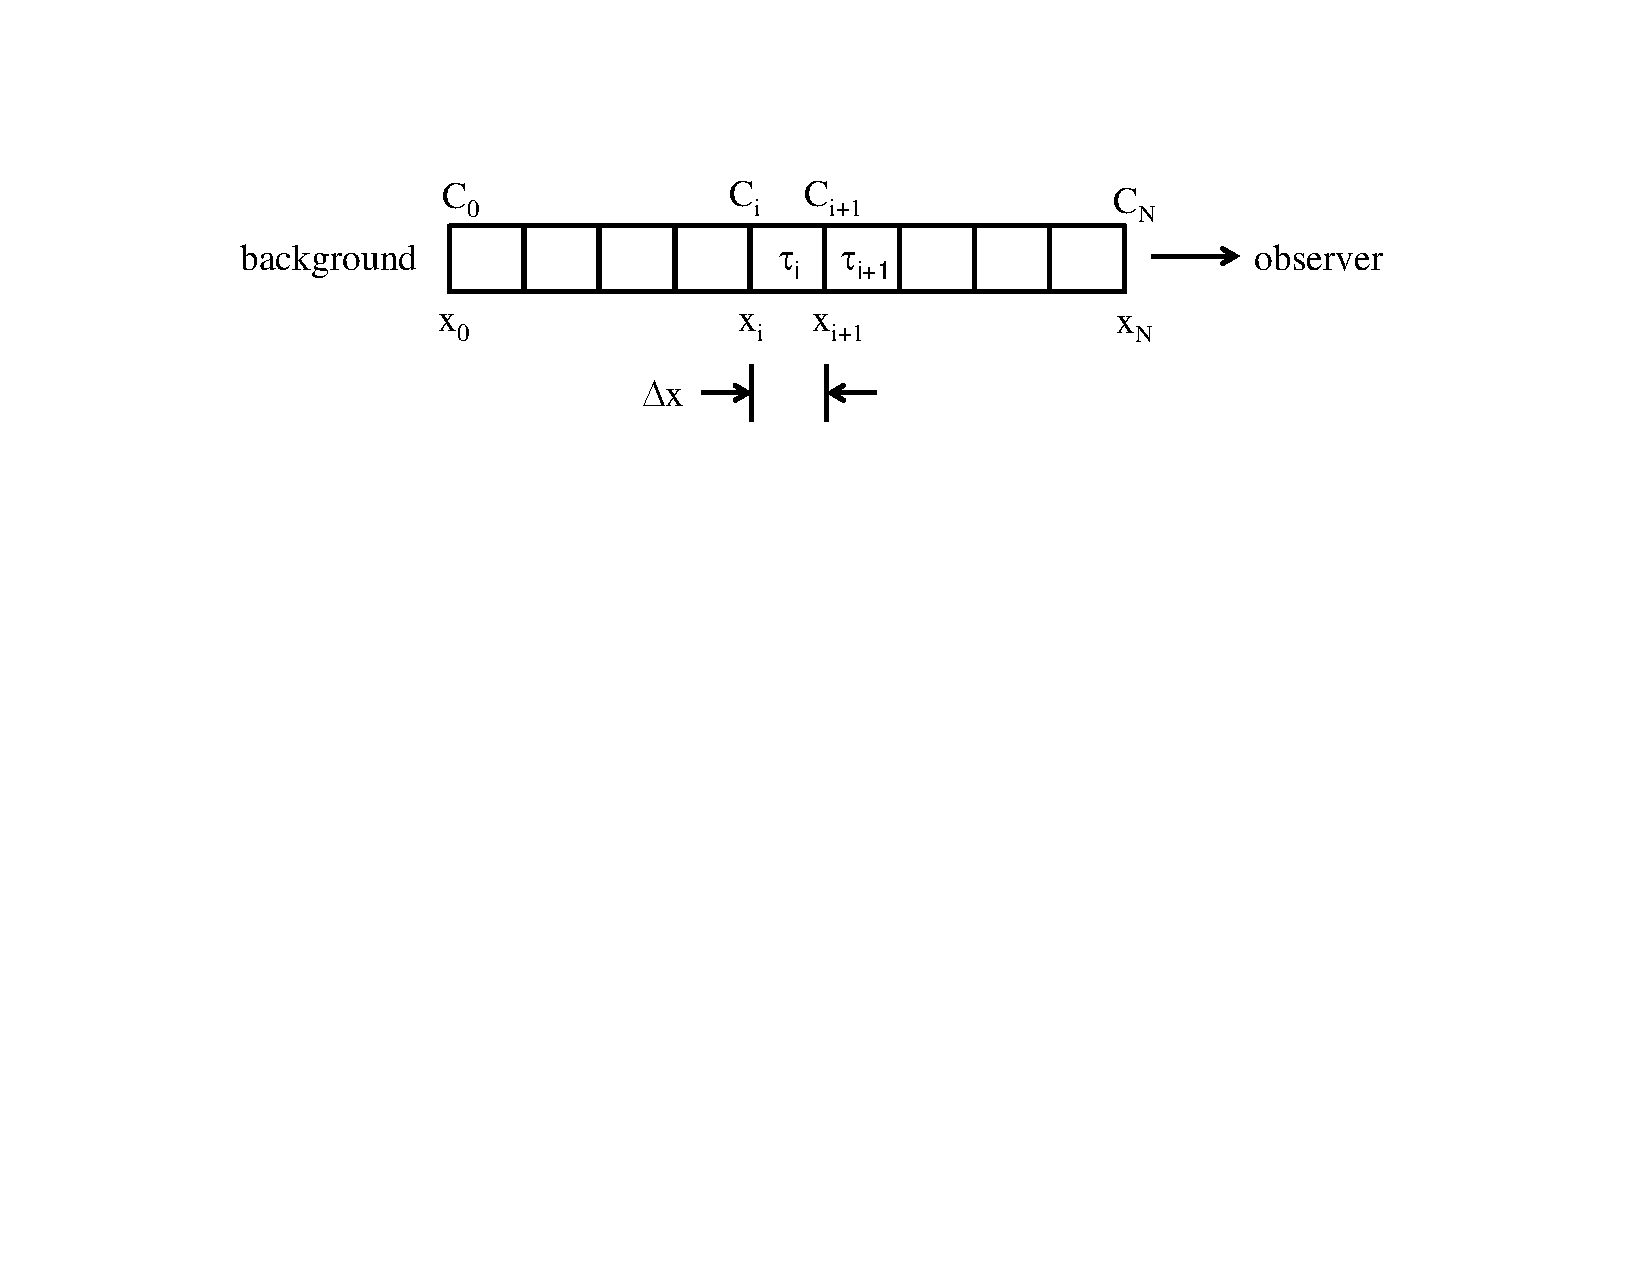
\includegraphics[width=5.0in]{\SMVfigdir/smoke_discrete_setup}
\end{center}
\caption[Setup for discretizing the equations used to model
radiance within a column of 3D smoke data.]{Setup for discretizing
the equations used to model radiance within a column of 3D smoke
data. The transparency across the interval from $x_i$ to $x_{i+1}$
is $\tau_i$. The transparency across the intervals from $x_i$ to
the observer is the product of individual transparencies or
$\tau_i\tau_{i+1}\cdots\tau_{N-1}$} \label{fig:smokediscretesetup}
\end{figure}

The optical depth, $\tau(a,b)$, defined in (\ref{eq:optdepth}) is
discretized using a Riemann sum  after defining sample points
$s_j=x_0+j\Delta s$ for $j=0$ to $N$ with spacing $\Delta
s=(x_N-x_0)/N$ to obtain

\begin{eqnarray}
\htau{i}=\tau(x_i,x_N)&=&\exp\left(-\int_{x_i}^{x_N}\sigma_t(s)\dx{s}\right)\approx\exp\left(-\sum_{j=i}^{N-1}\sigma_t(s_j)\Delta s\right)\\
&=&\prod_{j=i}^{N-1}\exp\left(-\sigma_t(s_j)\Delta s\right)=\prod_{j=i}^{N-1}\tau_j
\end{eqnarray}

\noindent where $\tau_j=\exp\left(-\sigma_t(s_j)\Delta s\right)$
represents the transparency over one discretization interval.
For~$i=N-1$~to~$0$, the optical depth $\htau{i}$ may be computed
recursively using
\begin{eqnarray}
\label{eq:tauhat_recurse}
\htau{i}&=&\htau{i+1}\tau_i
\end{eqnarray}
\noindent where the recursion is initiated with $\htau{N}=1$.
Substituting $1-\halpha{i}=\htau{i}$ and $1-\alpha_i=\tau_i$ into
(\ref{eq:tauhat_recurse}) gives
\begin{eqnarray}
1-\halpha{i}=(1-\halpha{i+1})(1-\alpha_i)=1-\halpha{i+1} - \alpha_i + \halpha{i+1}\alpha_i
\end{eqnarray}
which simplifies to
\begin{eqnarray}
\label{eq:alpha2}
\halpha{i}&=&\halpha{i+1} + (1-\halpha{i+1})\alpha_i
\end{eqnarray}

Similarly, the radiance given by the RTE solution $C(x_N)$ in
(\ref{eq:rtesoln}) may be discretized to obtain

\begin{eqnarray}
C_{N} = \htau{0}\,C_0 +
\sum_{i=0}^{N-1}\htau{i}\,\sigai{i}\,\Lei{i}\,\Delta x
\end{eqnarray}

\noindent where $\sigma_{a,i}=\sigma_a(x_i)$, $\Lei{i}=C_e(x_i)$,
$x_i=x_0+i\Delta x$ and $\Delta x=(x_N-x_0)/N$. This simplifies to

\begin{equation}
\label{eq:discrete_rte2}
C_N = \htau{0}C_0 + \sum_{i=0}^{N-1}\htau{i}\,\Leii{i}
\end{equation}

\noindent where $\Leii{i}=\sigma_{a,i}C_{e,i}\Delta x$.  If
$\Leii{i}$ is interpreted as the emitted color of the fire or
heated gas at location $i$ and $C_0$ is interpreted as the color
of the light source {\em behind}\ the smoke, then
(\ref{eq:discrete_rte2}) restated in words gives color seen by the
observer computed as a weighted average of source and emitted
colors where each weight is the optical depth from the observer to
the corresponding color location.  These emitted colors can be
determined from a blackbody temperature curve or from a colormap
meant to show variations in temperature in terms of color.


The terms in (\ref{eq:discrete_rte2}) are summed from back to
front meaning that the location of the $i=0$ term is farthest from
the observer, while the location of the $i=N-1$ term is closest.
We wish to perform this sum in reverse order, from front to back
so that the sum may be terminated early if additional
contributions would not significantly change the result.

Therefore, to compute $C_N$, let $\Chatjj{j}$ denote the partial
sum using terms $i=j$ through $i=N-1$ in the summation term in
(\ref{eq:discrete_rte2}).  Using this notation
$\hat{C}_N=\htau{0}C_0+\Chatjj{0}$ . Then

\begin{eqnarray}
\label{eq:recurse1}
\Chatjj{j} &= &\sum_{i=j}^{N-1}\htau{i}\,\Leii{i}\\
\label{eq:recurse2}
\Chatjj{j+1}     &= &\sum_{i=j+1}^{N-1}  \htau{i}\,\Leii{i}
\end{eqnarray}

Subtracting (\ref{eq:recurse2}) from (\ref{eq:recurse1}) and solving
for $\Chatjj{j}$ results in
\begin{eqnarray}
\label{eq:color}
\Chatjj{j}&=&\Chatjj{j+1}+\htau{j}\,\Leii{j}
\end{eqnarray}
The strategy then for volume rendering an image is for each pixel
in the 2D projected image to
\begin{enumerate}
\item convert the background radiance $C_0$ to a color,

\item convert the emitted radiances along the integration path to
colors and

\item form a weighted average of these colors using either
equation (\ref{eq:discrete_rte2}) or (\ref{eq:color}) where the
weights are optical depths obtained using (\ref{eq:alpha2}) .

\end{enumerate}
The conversion from radiance to color may be based on a blackbody
temperature curve if realistic flame colors are the goal or
arbitrary if only a qualitative view of the fire is the goal.
Equations (\ref{eq:alpha2}) and ({\ref{eq:color}) are equivalent
to the recursions presented in Ref.~\cite[Chapter 39]{gpugems} for
performing volume rendering.

% -------------------  A Solution using Slices ------------------------

\section{Implementation}
An algorithm for visualizing smoke and fire realistically consists of placing
planes within the solution domain and determining opacity and color
at various locations within these planes
using data generated by a fire model such as FDS.
The original smokeview algorithm placed planes exactly where data was recorded by FDS, either parallel to the XY, XZ or YZ axes planes or diagonally to two of these planes.
The new algorithm described below places planes in more general locations.
The increased flexibility
allows one to more easily reduce the amount of data accessed to draw smoke
Planes are placed perpendicular to the line of sight and are equally spaced though not necessarily the same same spacing as used by the underlying FDS grid.
This results in faster visualizations with the caveat that reduced data may result in less realistic visualizations.

\begin{enumerate}
\item Given spacing parameters parallel and perpendicular to the line of sight, place
equally spaced planes
through the data, each plane oriented perpendicular to the line of sight.
This is illustrated in Figure \ref{fig:smokeplanes}. Plane locations change as
the scene is moved.  By placing planes only where smoke is located, as illustrated in Figure \ref{fig:smokebox}, faster visualizations result.

\begin{figure}[bph]
\begin{center}
\includegraphics[height=3.0in]{../SMV_USER_GUIDE/SCRIPT_FIGURES/smokegeom_fullbox}
\end{center}
\caption{Planes are placed within the entire solution domain.  The planes are equally spaced and oriented perpendicular to the line of sight.}
\label{fig:smokeplanes}
\end{figure}


\begin{figure}[bph]
\begin{center}
\begin{tabular}{cc}
\includegraphics[height=3.0in]{../SMV_USER_GUIDE/SCRIPT_FIGURES/smokegeom_smoke}
\includegraphics[height=3.0in]{../SMV_USER_GUIDE/SCRIPT_FIGURES/smokegeom_smokebox}
\end{tabular}
\end{center}
\caption{Planes are placed only where smoke is located resulting in faster visualizations.}
\label{fig:smokebox}
\end{figure}

\item Each data plane must now be triangulated, divided into a series of equally sized triangles (except for triangles that border the edge of the polygon). To do this
    a 2D coordinate
    system is constructed for the planar polygon. As illustrated in Figure \ref{fig:smoketriangulate}, let $\vvec{u}$ be a vector corresponding to the longest
    polygonal side.  Let $\vvec{v}$ be a vector corresponding to the side clockwise (from the point of view of the observer) from $\vvec{u}$ .

      Orthogonal unit length vectors, $\vvec{s}$ and $\vvec{t}$, are formed using

      \begin{eqnarray*}
    \vvec{s}&=&\vvec{u}/||\vvec{u}||,\\
    \vvec{t}&=&(\vvec{s} \times \vvec{\hat{v}}) \times \vvec{\hat{v}}
    \end{eqnarray*}
    where $\vvec{\hat{v}}=\vvec{v}/||\vvec{v}||$.

\begin{figure}[bph]
\begin{center}
\begin{tabular}{cc}
\includegraphics[height=3.5in]{../../../fig/smv/figures/smokegeom_5p5265poly}
\includegraphics[height=3.5in]{../../../fig/smv/figures/smokegeom_triangulation}
\end{tabular}
\end{center}
\caption[smoke]
{smoke}
\label{fig:smoketriangulate}
\end{figure}

\item Determine coordinates, $(a_i,b_i)$, for each polygonal vertex, $p_i$, in terms of vectors $\vvec{s}$ and $\vvec{t}$ using

\begin{eqnarray*}
    a_i&=&(p_i-x_0) \cdot \vvec{s}\\
    b_i&=&(p_i-x_0) \cdot \vvec{t}
\end{eqnarray*}

where $x_0$ is translated from $p_0$ in the polygonal plane so that all $a_i$ and $b_i$ are positive.

\item For a spacing parameter $\Delta$, the polygon is triangulated by
first forming vertices $t_{ij}$ for $0\le i\le M$ and
$0\le j\le N$ where

\begin{eqnarray*}
t_{ij}&=&x_0 + i\vvec{s} + j \vvec{t}\\
M&=&\max{a_i/\Delta}\\
N&=&\max{b_i/\Delta}
\end{eqnarray*}
and then forming triangles $(t_{ij},t_{i+1,j},t_{i+1,j+1}), (t_{ij},t_{i+1,j+1},t_{i,j+1}) $ from these vertices. Note, if all three vertices of a triangle are outside the polygon it is ignored.  If one or two vertices are outside the polygon they are moved to the closest point on the polygon.

\end{enumerate}

A slice rendering algorithm for visualizing smoke consists of
splitting the RTE across individual slice planes within a single
mesh.  The 3D computational domain is partitioned into a series of
2D slices.  The RTE is then solved on each slice.  Each slice
solution only accounts for conditions between adjacent slices.
The individual partially transparent slice solutions are then
combined using video hardware to form the final image.   Problems
can occur with numerical round off error if two slices are too
close together.

The slice orientation
is chosen to be the one most perpendicular to the viewer's line of
sight.  The opacity at each vertex is computed using the
distance between adjacent planes and soot density
data computed by the fire model.  Opacities are adjusted if the distance
between planes is different than the spacing parameter used to compute the original opacity.  Opacity data is
computed and compressed using run length encoding as a
preprocessing step and decompressed as each frame is
displayed.



% -------------------  Computing Color ------------------------

\subsection{Computing Color}

Smokeview visualizes smoke and fire by drawing a series of triangles in equally spaced parallel planes.
Color for these triangles are assigned by mapping temperature or hrrpuv (heat release per unit volume) values
to color such as with a color map illustrated in Figure \ref{fig:colormaps}.
Transparency for these triangles is assigned using soot density, the greater the soot density, the more opaque the triangle.

The example color map in Fig.
\ref{fig:colormaps} is split into two parts.  The left half is used
for coloring non-burning regions, the right half is used for coloring burning regions.
An hrrpuv cutoff value denoted ${\rm hrrpuv}_{\rm cutoff}$ is used to
distinguish these two regions.
If an hrrpuv value is below the cutoff,
smoke is drawn using colors from the left half of the color map, while if an hrrpuv value is greater than the cutoff,
fire is drawn using colors from the right half of the color map.  The color map is defined as a table
of 256 red, green, blue color triplets.  A formula giving a color index for a given hrrpuv value is given by

\newcommand{\hrr}{{\rm hrr}}
\newcommand{\hrrcutoff}{{\rm hrr}_{\rm cutoff}}
\newcommand{\hrrmax}{{\rm hrr}_{\rm max}}

\begin{eqnarray}
\mbox{color index}=\left\{
\begin{array}{ll}
  127\frac{\hrr}{\hrrcutoff} & 0 \le \hrr \le \hrrcutoff \\
  127 + 128\frac{\hrr-\hrrcutoff}{\hrrmax-\hrrcutoff} & \hrrcutoff \le \hrr \le \hrrmax
\end{array}
\right.
\end{eqnarray}

\begin{figure}[bph]
\begin{center}

\includegraphics[width=5.0in]{\SMVfigdir/colorbar_fire2}
\end{center}
\caption[Example colormap used for converting temperature or hrrpuv values to color.]
{Example colormap used for converting temperature or hrrpuv values to color.}
\label{fig:colormaps}
\end{figure}

% -------------------  Computing Opacity ------------------------

\subsection{Computing Opacity}
Consider a ray traveling from the background to the
observer through intervening smoke. Light is absorbed or scattered
by the smoke as the ray passes through each slice plane. Emission effects
are accounted for by coloring the smoke.  Scattering effects
are accounted for by the total mass
extinction coefficient.  Light losses are assumed to be from both
absorption and scattering. Obscuration or opacity is computed along each
ray one grid plane at a time, using the Beer-Lambert law as
follows.  The $\alpha=1-\tau$ values are pre-computed by FDS using
the Beer-Lambert law~\cite{Siegel:2001}

\begin{equation}
\label{eq:alpha}
\alpha=1-\exp(-\sigma_t\Delta x)
\end{equation}

\noindent for the view direction down the $x$~axis
where $\Delta x$ is the distance between two grid planes and
$\sigma_t=\sigma_a+\sigma_s$ is the total mass extinction
coefficient.  The Beer-Lambert law is an empirical relationship
relating light absorption to the material properties of the medium
the light is travelling through, in this case soot or smoke.

The $\alpha$ parameter in (\ref{eq:alpha}) is used by
OpenGL~\cite{OpenGLRed} to blend smoke planes with the current
background.  The $\alpha$ parameter used here also represents an
opacity, 0.0, for completely transparent, and 1.0 for completely
opaque.

The absorption parameter, $\alpha$, needs to be adjusted when the spacing is different than $\Delta x$, 
(the spacing FDS uses to pre-compute $\alpha$ terms).
The adjusted $\hat{\alpha}$ for a new spacing $\Delta\hat{x}$ is given by

\begin{equation}
\label{eq:alphahat}
\hat{\alpha}=1-(1-\alpha)^{\Delta\hat{x}/\Delta x}
\end{equation}

after noting that

\begin{eqnarray}
1-\hat{\alpha}=\exp(-\sigma_t\Delta\hat{x})=\exp(-\sigma_t\Delta
x)^{\Delta\hat{x}/\Delta x}=(1-\alpha)^{\Delta\hat{x}/\Delta x}
\end{eqnarray}

% -------------------  Future Work ------------------------

\section{Future Work}
This \paper\ describes the algorithms Smokeview uses to display
smoke and fire using physics based algorithms. These algorithms
may be improved in several ways. Presently, only radiation from
soot is used to visualize smoke. The gray gas assumption may be
relaxed by solving the RTE for several wavelength bands (as may be
done by FDS) and combining the results. The RTE line integration
needs to terminate at the first solid object encountered (FDS
OBST) rather than the far side of the data mesh. The computational
efficiency may be improved by implementing algorithms to skip over
regions with little or no smoke. Research on unstructured
geometries for future incorporation into FDS may also lead to
better visualization. Finally, flame color computations may be
made more quantitative by using a transfer function relating
temperature to color that is physics based rather than an assumed
color map.
